\documentclass{article}
\usepackage[a4paper, margin=3cm]{geometry}
\usepackage[utf8]{inputenc}
\usepackage{amsmath}
\usepackage{amssymb}
\usepackage{verbatim}
\usepackage{dirtytalk}
\usepackage{calc}
% \usepackage{tikz}
\usepackage{pgfplots}
\usepackage{titlesec}
\usepackage{wrapfig}
\usepackage{fancyhdr}
\usepackage{xcolor}
\usepackage[hidelinks]{hyperref}
\usepackage[inline]{enumitem}

\listfiles

\titleclass{\section}{top}
\newcommand\sectionbreak{\clearpage}

\fancypagestyle{plain}{
    \fancyhf{}
    \lhead{ CS4099 Notes }
    \rhead{ Georg Wölflein }
    \cfoot{ \thepage }
}
\pagestyle{plain}


\pgfplotsset{compat=1.16}
\pgfplotsset{every axis plot post/.append style={mark=none}}
\usetikzlibrary{calc, patterns}
\usetikzlibrary{hobby}
\usetikzlibrary{decorations.markings}
\usepgfplotslibrary{external, fillbetween}
\tikzexternalize[prefix=figures/]

\definecolor{darkcyan}{rgb}{0.0, 0.55, 0.55}

\title{CS4099}
\author{\vspace{-5ex}}
\date{\vspace{-5ex}}

\renewcommand\vec{\mathbf}
\newcommand{\norm}[1]{\left\lVert#1\right\rVert}

\pgfdeclarelayer{pre main}
\begin{document}

%\maketitle

\section{Week 2}

\paragraph{Control and output spaces}
The control space for robots is the wheels, and for neural nets the weights and biases.
The output space for robots is the movement/travel in the 2D obstacle space, and for neural nets the activation of the output layer.

\paragraph{The cost function}
Consider the output space
$$
    \vec{y} =
    \begin{bmatrix}
        y_{1} \\
        y_{2}
    \end{bmatrix}
    \in \mathbb{R}^2
.$$
The current weight configuration in the control space
$$
    \vec{w} =
    \begin{bmatrix}
        w_{1} \\
        w_{2} \\
        w_{3}
    \end{bmatrix}
    \in \mathbb{R}^3
$$
produces the initial output $\textcolor{blue}{i} \in \textbf{y}$. Our goal is $\textcolor{red}{g}  \in \textbf{y}$.




\begin{figure}[h]

    \begin{tikzpicture}

        \draw[thick, <->]
            (0, 5.5) node(y2line)[above] {$y_2$}
            |- (10, 0) node(y1line)[right] {$y_1$};

        \coordinate (i) at (2, 3);
        \coordinate (g) at (9, 3);
        \coordinate (frac_progress) at ($(i)!2cm!(g)$);
        \coordinate (frac_line_a) at (frac_progress |- y2line);
        \coordinate (frac_line_b) at (frac_progress |- y1line);

        \coordinate (dw_1) at ($(i)+(45:2cm)$);
        \coordinate (dw_2) at ($(i)+(-20:2cm)$);
        \coordinate (dw_3) at ($(i)+(-60:-2cm)$);
        \coordinate (dw_3_actual) at ($(i)+(-60:2cm)$);

        \draw[->] (i) -- (dw_1) node[above left] {$\frac{\delta \vec{y}}{\delta w_1}$};
        \draw[->] (i) -- (dw_2) node[below] {$\frac{\delta \vec{y}}{\delta w_2}$};
        \draw[->] (i) -- (dw_3) node[above] {$\frac{\delta \vec{y}}{\delta w_3}$};
        \draw[->, cyan] (i) -- (frac_progress);

        \draw[dotted, cyan] (frac_line_a) -- (frac_line_b);
        \draw[dotted] (dw_1 |- y2line) -- (dw_1 |- y1line);
        \draw[dotted] (dw_2 |- y2line) -- (dw_2 |- y1line);
        \draw[dotted] (dw_3_actual |- y2line) -- (dw_3_actual |- y1line);

        \draw[dashed] (i) -- (dw_1) -- (g);
        \draw[dashed] (i) -- (dw_2) -- (g);
        \draw[dashed] (i) -- (dw_3_actual) -- (g);
        \draw[->, dashed, cyan] (i) -- (g);

        \fill[blue] (i) circle (2pt) node[left] {$i$};
        \fill[red] (g) circle (2pt) node[right] {$g$};

    \end{tikzpicture}

    \caption{Diagram of the output space.}

\end{figure}



We define the cost function as
\begin{equation}
    C\left( \vec{w} \right) = \frac{\text{fractional progress}}{\text{total Euclidean distance}}.
\end{equation}

The \textcolor{cyan}{straight line goal-connecting path} would minimize the Euclidean distance while maximizing the fractional progress.




\section{Week 3}

\subsection{Research}
\paragraph{Simulated annealing}
This refers to a process that will temporarily accept sub-optimal (worse) values in hopes of overcoming local maxima, to reach better local minima.

\paragraph{Adam optimizer}
The name means \say{ADAptive Moment estimation}.
Instead of using a global learning rate (as in SGD), Adam \say{computes individual adaptive learning rates for different parameters from estimates of first and second moments of the gradients} \cite{adam}, i.e. the mean and variance.

\paragraph{The stripe problem in literature}
To do

\subsection{A problem that always achieves a point on the goal line (gradient of weights are at right angle)}

Consider the neural network below. Note that it does not have an activation function.

\begin{figure}[h]
    \begin{center}
        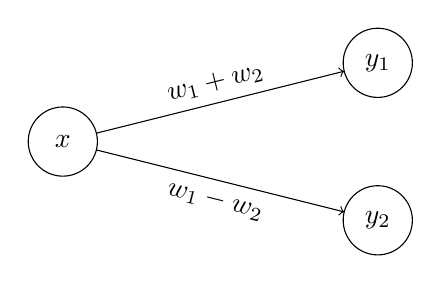
\begin{tikzpicture}
            [
                neuron/.style = {draw, circle, minimum size=25pt, inner sep=0pt, outer sep=0pt},
            ]
            
            \node [neuron] (x)  at (0,0) {$x$};
            \node [neuron] (y1) at (4,1) {$y_1$};
            \node [neuron] (y2) at (4,-1) {$y_2$};
            \draw[->] (x) -- (y1) node[midway, above, sloped] {$w_1 + w_2$};
            \draw[->] (x) -- (y2) node[midway, below, sloped] {$w_1 - w_2$};
        \end{tikzpicture}
    \end{center}
    \caption{The neural network.}
\end{figure}

Here we have
\begin{equation*}
    \vec{y}(x; \vec{w}) = 
    \begin{bmatrix}
        w_1 + w_2 \\
        w_1 - w_2
    \end{bmatrix}
    x
\end{equation*}
with the derivative
\begin{equation*}
    \frac{\partial \vec{y}}{\partial \vec{w}}
    =
    \begin{bmatrix}
        \frac{\partial y_1}{\partial w_1} & \frac{\partial y_1}{\partial w_2} \\
        \frac{\partial y_2}{\partial w_1} & \frac{\partial y_2}{\partial w_2}
    \end{bmatrix}
    =
    \begin{bmatrix}
        1 & 1 \\
        1 & -1
    \end{bmatrix}
    x.
\end{equation*}

For
$x = 1$,
let our goal be $\vec{g} = \begin{bmatrix} 10 \\ 2 \end{bmatrix}$
and the initial weight configuration be
$\vec{w} = \begin{bmatrix} 3 \\ 1 \end{bmatrix}$.
This leads to the current position $\vec{p} = \begin{bmatrix} 4 \\ 2 \end{bmatrix}$ in output space.

Say we want to achieve $\frac{1}{6}$ fractional progress, so we aim to achieve the point $\vec{q}$ at the intersection of the fractional progress line with the goal line in the diagram of Fig. \ref{fig:week3fractionlprogress}. 


\begin{figure}[h]
    \centering
    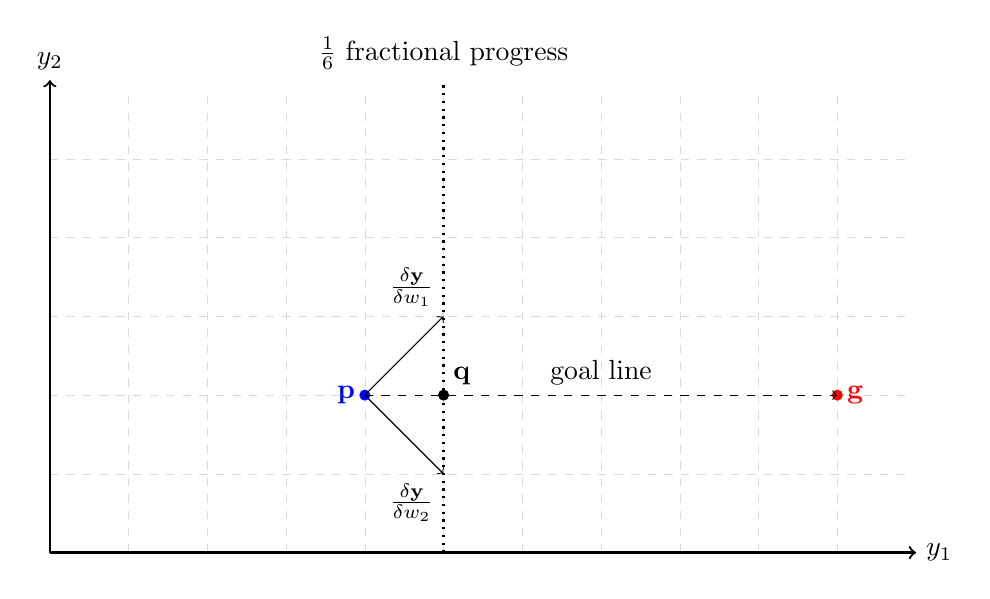
\begin{tikzpicture}
        
        \draw[help lines, color=gray!30, dashed] (0, 5.9) grid (10.9, 0);
        \draw[thick, ->] (0, 0) -- (11, 0) node[right] {$y_1$};
        \draw[thick, ->] (0, 0) -- (0, 6) node[above] {$y_2$};
        
        \coordinate (p) at (4, 2);
        \coordinate (g) at (10, 2);
        \coordinate (dw_1) at (1, 1);
        \coordinate (dw_2) at (1, -1);
        \coordinate (q) at (5, 2);
        
        \fill[blue] (p) circle (2pt) node[left] {$\vec{p}$};
        \fill[red] (g) circle (2pt) node[right] {$\vec{g}$};
        \fill (q) circle (2pt) node[above right] {$\vec{q}$};
        
        \draw[->] (p) -- +(dw_1) node[above left] {$\frac{\delta \vec{y}}{\delta w_1}$};
        \draw[->] (p) -- +(dw_2) node[below left] {$\frac{\delta \vec{y}}{\delta w_2}$};
        \draw[thick, dotted] (5, 0) -- (5, 6) node[above] {$\frac{1}{6}$ fractional progress};
        \draw[->, dashed] (p) -- (g) node[midway, above] {goal line};

    \end{tikzpicture}

    \caption{Diagram of the weights' partial derivatives in output space along with the sub-goal.}
    \label{fig:week3fractionlprogress}
\end{figure}

Now we need to find out by how much we need to update $\vec{w}$. In other words, we need to find $\vec{a} \in \mathbb{R}^2$ so that after
\begin{equation}
    \label{update_w}
    \vec{w} \leftarrow \vec{w} + \vec{a}
\end{equation}
we get
\begin{equation*}
    \vec{y}(1; \vec{w}) =
    \begin{bmatrix}
        4 \\
        2
    \end{bmatrix} + 
    \begin{bmatrix}
        1 \\
        0
    \end{bmatrix}.
\end{equation*}

This is equivalent to finding the vector $\vec{a} = \begin{bmatrix} a_1 \\ a_2 \end{bmatrix}$ that satisfies
\begin{align*}
    \begin{bmatrix}
        1 \\
        0
    \end{bmatrix}
    &=
    \frac{\partial \vec{y}}{\partial \vec{w}} \cdot \vec{a}
    \\
    &=
    a_1
    \frac{\partial \vec{y}}{\partial w_1}
    +
    a_2
    \frac{\partial \vec{y}}{\partial w_2}
    \\
    &=
    a_1
    \begin{bmatrix}
        1 \\
        1
    \end{bmatrix}
    +
    a_2
    \begin{bmatrix}
        1 \\
        -1
    \end{bmatrix},
\end{align*}
so
\begin{align*}
    a_1 = a_2 = \frac{1}{2} \\
    \vec{a} =
    \frac{1}{2}
    \begin{bmatrix}
        1 \\
        1
    \end{bmatrix}.
\end{align*}

Using (\ref{update_w}), we update $\vec{w}$ to
\begin{equation*}
    \vec{w}
    \leftarrow
    \begin{bmatrix}
        3 \\
        1
    \end{bmatrix}
    +
    \frac{1}{2}
    \begin{bmatrix}
        1 \\
        1
    \end{bmatrix}
    =
    \frac{1}{2}
    \begin{bmatrix}
        7 \\
        3
    \end{bmatrix}.
\end{equation*}


Now let's see what we get for the new $\vec{q}$ in this updated system:
\begin{equation*}
    \vec{q} =
    \vec{y}(1; \vec{w}) =
    \begin{bmatrix}
        w_1 + w_2 \\
        w_1 - w_2
    \end{bmatrix} = 
    \frac{1}{2}
    \begin{bmatrix}
        7+3 \\
        7-3
    \end{bmatrix}
    =
    \begin{bmatrix}
        5 \\
        2
    \end{bmatrix}
\end{equation*}
which is correct (see diagram).

\paragraph{Remarks:}
In this very simple example, we can use linear algebra to deterministically reach our sub-goal. 
However, as soon as we have three weights, there will be more than one possible vector $\vec{a} \in \mathbb{R}^3$ that achieves the sub-goal. 
Are there any drawbacks for choosing a particular $\vec{a}$ over another, if there are multiple options?

Furthermore, this network is so simple that the partial derivatives of the weights with respect to the output space aren't dependent on the weights themselves. However, in a \say{real} neural network, the gradients will influence each other because they depend on the weights. What happens in that case? (This question is examined in the next section.)

\subsection{When gradients are dependent on other weights}
Consider the neural network below. It uses the ReLU activation function.

\begin{figure}[h]
    \begin{center}
        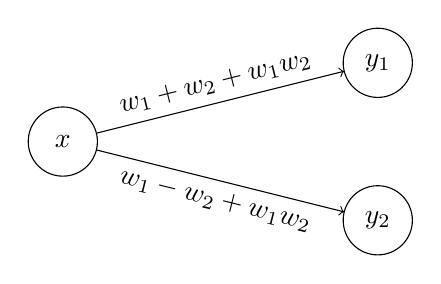
\begin{tikzpicture}
            [
                neuron/.style = {draw, circle, minimum size=25pt, inner sep=0pt, outer sep=0pt},
            ]
            
            \node [neuron] (x)  at (0,0) {$x$};
            \node [neuron] (y1) at (4,1) {$y_1$};
            \node [neuron] (y2) at (4,-1) {$y_2$};
            \draw[->] (x) -- (y1) node[midway, above, sloped] {$w_1 + w_2 + w_1 w_2$};
            \draw[->] (x) -- (y2) node[midway, below, sloped] {$w_1 - w_2 + w_1 w_2$};
        \end{tikzpicture}
    \end{center}
    \caption{The neural network.}
\end{figure}

Here we have
\begin{equation*}
    \vec{y}(x; \vec{w}) = 
    \begin{bmatrix}
        \max \left( 0, w_1 + w_2 + w_1 w_2 \right) \\
        \max \left( 0, w_1 - w_2 + w_1 w_2 \right)
    \end{bmatrix}
    x
\end{equation*}
with the derivative
\begin{equation*}
    \frac{\partial \vec{y}}{\partial \vec{w}}
    =
    \begin{bmatrix}
        \max(0, w_2 + 1) & \max(0, w_1 + 1) \\
        \max(0, w_2 + 1) & \max(0, w_1 - 1)
    \end{bmatrix}
    x.
\end{equation*}

For
$x = 1$,
let our goal be $\vec{g} = \begin{bmatrix} 9 \\ 1 \end{bmatrix}$
and the initial weight configuration be
$\vec{w} = \begin{bmatrix} 1 \\ 1 \end{bmatrix}$.
This leads to the current position $\vec{p} = \begin{bmatrix} 3 \\ 1 \end{bmatrix}$ in output space.


\begin{figure}[h]
    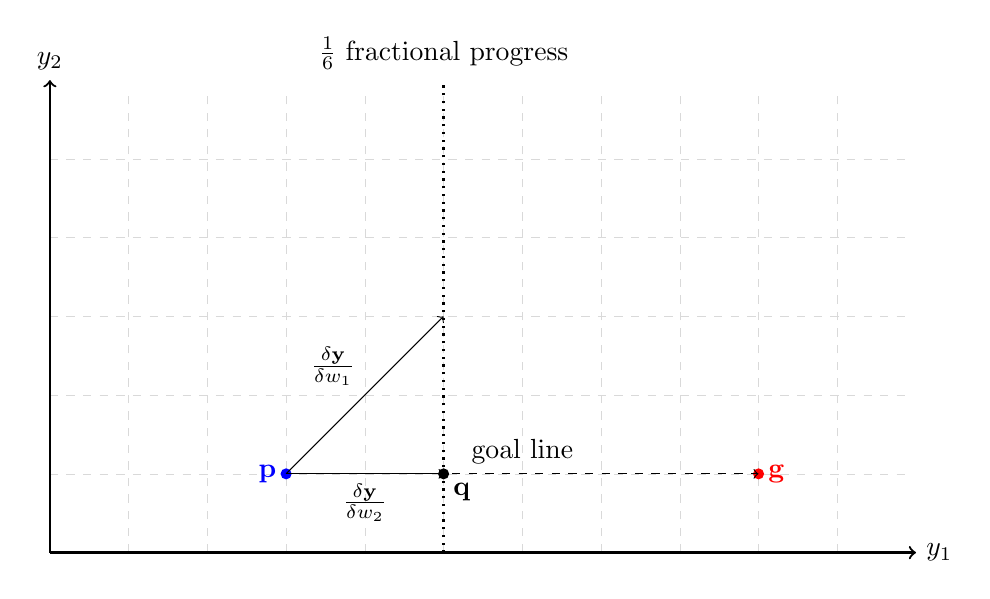
\begin{tikzpicture}
        
        \draw[help lines, color=gray!30, dashed] (0, 5.9) grid (10.9, 0);
        \draw[thick, ->] (0, 0) -- (11, 0) node[right] {$y_1$};
        \draw[thick, ->] (0, 0) -- (0, 6) node[above] {$y_2$};
        
        \coordinate (p) at (3, 1);
        \coordinate (g) at (9, 1);
        \coordinate (dw_1) at (2, 2);
        \coordinate (dw_2) at (2, 0);
        \coordinate (q) at (5, 1);
        
        \fill[blue] (p) circle (2pt) node[left] {$\vec{p}$};
        \fill[red] (g) circle (2pt) node[right] {$\vec{g}$};
        \fill (q) circle (2pt) node[below right] {$\vec{q}$};
        
        \draw[->] (p) -- +(dw_1) node[midway, above left] {$\frac{\delta \vec{y}}{\delta w_1}$};
        \draw[->] (p) -- +(dw_2) node[midway, below] {$\frac{\delta \vec{y}}{\delta w_2}$};
        \draw[thick, dotted] (5, 0) -- (5, 6) node[above] {$\frac{1}{6}$ fractional progress};
        \draw[->, dashed] (p) -- (g) node[midway, above] {goal line};

    \end{tikzpicture}

    \caption{Diagram of the weights' partial derivatives in output space along with the sub-goal.}
\end{figure}

Just looking at the diagram, one could guess to update the weights as follows to achieve $\vec{q}$:
\begin{equation*}
    \vec{w} \leftarrow \vec{w} +
    \begin{bmatrix}
        0 \\
        1
    \end{bmatrix}.
\end{equation*}
Using $\vec{w} = \begin{bmatrix} 1 \\ 2 \end{bmatrix}$, we calculate the new output
\begin{equation*}
    \vec{y}(1; \vec{w})
    = 
    \begin{bmatrix}
        \max \left( 0, 1 + 2 + 2 \right) \\
        \max \left( 0, 1 - 2 + 2 \right)
    \end{bmatrix}
    =
    \begin{bmatrix}
        5 \\
        3
    \end{bmatrix}
\end{equation*}
which is \textit{not} our sub-goal $\vec{p}$! The reason for this is that unlike the previous network, the partial derivative $\frac{\partial \vec{y}}{\partial w_1}$ is dependent on the value of $w_2$ and vice-versa.

\paragraph{Remarks:}
When the partial derivatives are functions of each other (i.e. depend on each other), we can't use simple linear algebra in order to find the combination of the weights to achieve a specific subgoal. 
This makes intuitive sense, because if it were possible, we could simply choose the goal as our subgoal and expect to use linear algebra to find the optimum weight configuration which would eliminate the need for training neural networks.

\subsection{A problem with an unrealizable goal line, but realizable goal}
Did not find a good example yet.


\section{Week 5}

\subsection{Research}

\paragraph{Radial basis function}
A radial basis function is a real-valued function $f$ that satisfies the property $f(\vec{x}) = f(\norm{\vec{x}})$. 
RBFs are used as a kernel in SVMs. 
They are infinitely differentiable.

Two commonly used RBFs are the Gaussian function
$$ f(x) = e^{-x^2} $$
and the bump function
$$ f(x) = 
\begin{cases}
    e^{-\frac{1}{1-x^2}} & \text{for $-1<x<1$} \\
    0 & \text{otherwise}.
\end{cases}
$$

\subsection{Replicating the simple neural network with the shallow excitation gradient}
\label{sec:week5:shallownet}
Consider the very simple neural network below. 
\begin{figure}[h]
    \begin{center}
        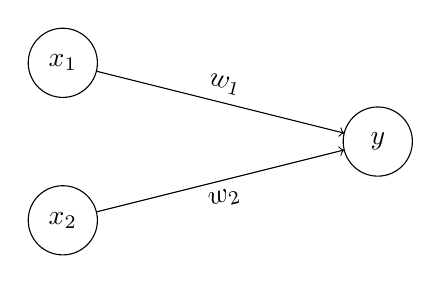
\begin{tikzpicture}
            [
                neuron/.style = {draw, circle, minimum size=25pt, inner sep=0pt, outer sep=0pt},
            ]
            
            \node [neuron] (x1)  at (0,2) {$x_1$};
            \node [neuron] (x2) at (0,0) {$x_2$};
            \node [neuron] (y) at (4,1) {$y$};
            \draw[->] (x1) -- (y) node[midway, above, sloped] {$w_1$};
            \draw[->] (x2) -- (y) node[midway, below, sloped] {$w_2$};
        \end{tikzpicture}
    \end{center}
    \caption{The neural network.}
    \label{fig:week5:shallownet}
\end{figure}

The output neuron's excitation is given by 
\begin{equation*}
    y(\vec{x}; \vec{w}, b) = \vec{w} \vec{x} + b.
\end{equation*}

Consider the two points in input space
$\vec{a} = 
\begin{bmatrix}
    0.6 \\ 0.4
\end{bmatrix}$
and
$\vec{b} = 
\begin{bmatrix}
    1 \\ 0.4
\end{bmatrix}$
with the targets $y(\vec{a}) = 0.2$ and $y(\vec{b}) = 0.8$.

The current weight configuration should be such that the hyperplane in output space of the 0.5 excitation line should be given by $x_1=0.5$.
Furthermore, the current activations should be $y(\vec{a}) = 0.51$ and $y(\vec{b}) = 0.55$ such that we get the configuration outlined in Fig. \ref{week5:initial}.
\begin{figure}[h]
    
    \centering

    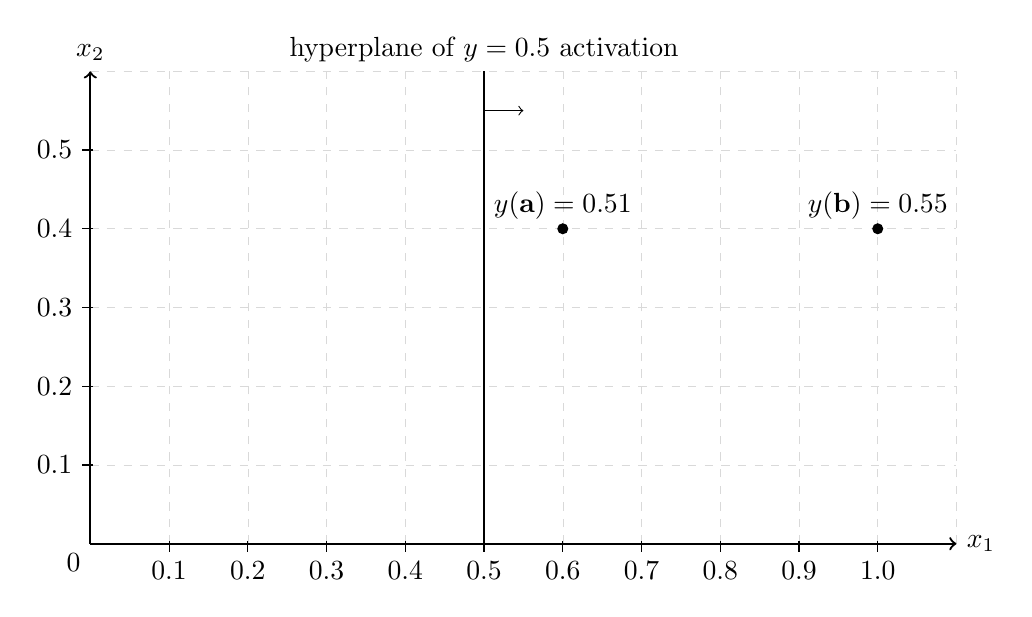
\begin{tikzpicture}[x=10cm,y=10cm]
        
        \draw[help lines, color=gray!30, dashed] (0, .6) grid (1.1, 0);
        \draw[thick, ->] (0, 0) -- (1.1, 0) node[right] {$x_1$};
        \draw[thick, ->] (0, 0) -- (0, .6) node[above] {$x_2$};
        \foreach \x in {0.1, 0.2, 0.3, 0.4, 0.5, 0.6, 0.7, 0.8, 0.9, 1.0 }
     		\draw (\x,1pt) -- (\x,-3pt)
            node[anchor=north] {\x};
        \foreach \y in {0.1, 0.2, 0.3, 0.4, 0.5 }
            \draw (1pt,\y) -- (-3pt,\y)
           node[anchor=east] {\y};
        \draw (0, 0) node[below left] {0};
        
        \draw (0.5, 0) -- (.5, .6) node[above] {hyperplane of $y=0.5$ activation};
        
        \coordinate (a) at (.6, .4);
        \coordinate (b) at (1, .4);
        
        \fill (a) circle (2pt) node[above] {$y(\vec{a})=0.51$};
        \fill (b) circle (2pt) node[above] {$y(\vec{b})=0.55$};

        \draw[->] (.5, .55) -- (.55, .55);
    \end{tikzpicture}

    \caption{The initial configuration with the hyperplane. The arrow is pointing in the direction of increasing activation.}
    \label{week5:initial}
\end{figure}

After some experimentation, it was established that this configuration can be achieved using
$\vec{w} = \begin{bmatrix}
    0.1 \\ 0.0005
\end{bmatrix}$
and $b = 0.45$ thus leading to the function
\begin{equation*}
    y(\vec{x}) = 0.1 x_1 + 0.0005 x_2 + 0.45.
\end{equation*}

\paragraph{Remarks:}
To get a gradient this shallow, it was necessary to introduce a third parameter $b$. 
We need to investigate whether we can call it a \say{non-trainable variable}, so we effectively only have two weights.

\section{Week 6}

\subsection{The hyperplanes of radial basis activation functions}
Consider the radial basis function
\begin{equation}
    \label{eq:week6:rbf}
    \phi(x) = e^{-x^2}
\end{equation}
with the graph pictured in Fig. \ref{fig:week6:rbf:plot}.

\begin{figure}[h]
    \centering
    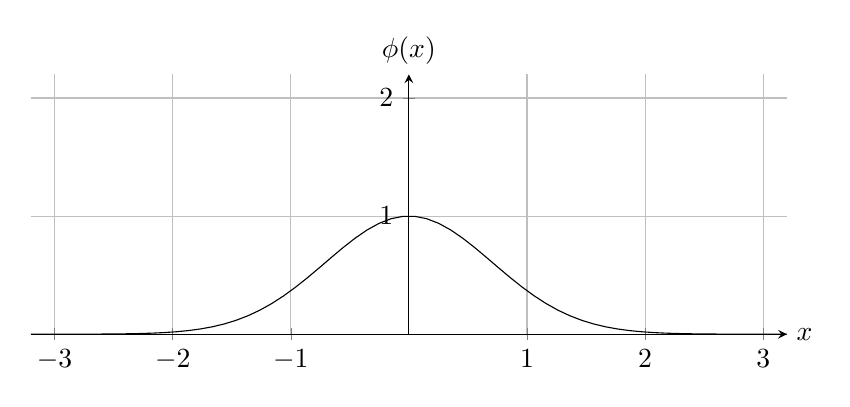
\begin{tikzpicture}
        \begin{axis}[
            x=1.5cm,
            y=1.5cm,
            axis lines=center,
            xlabel={$x$}, xlabel style={anchor=west},
            ylabel={$\phi(x)$}, ylabel style={anchor=south},
            ymin=0, ymax=2.2,
            xmin=-3.2, xmax=3.2,
            grid,
            samples=100,
            xtick={-3,...,3},
            ytick={0, 1, 2}
        ]
            \addplot[black] {exp(-x*x)};
        \end{axis}
    \end{tikzpicture}
    \caption{Plot of the radial basis activation function.}
    \label{fig:week6:rbf:plot}
\end{figure}

To examine the hyperplanes corresponding to this activation function, consider the very simple neural network given in Fig. \ref{fig:week6:rbf:neuralnet}. 
\begin{figure}[h]
    \centering
    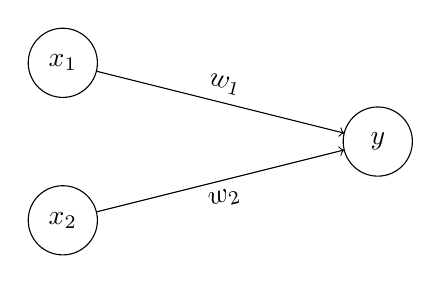
\begin{tikzpicture}
        [
            neuron/.style = {draw, circle, minimum size=25pt, inner sep=0pt, outer sep=0pt},
        ]
        
        \node [neuron] (x1)  at (0,2) {$x_1$};
        \node [neuron] (x2) at (0,0) {$x_2$};
        \node [neuron] (y) at (4,1) {$y$};
        \draw[->] (x1) -- (y) node[midway, above, sloped] {$w_1$};
        \draw[->] (x2) -- (y) node[midway, below, sloped] {$w_2$};
    \end{tikzpicture}
    \caption{The neural network.}
    \label{fig:week6:rbf:neuralnet}
\end{figure}

For simplicity, we set $w_1=w_2=1$. 
The output neuron's activation is then given by 
\begin{equation*}
    y(\vec{x}) = \phi(x_1 + x_2).
\end{equation*}

To find the equations of the hyperplanes, we set the output to 0.5, so
\begin{align*}
    \frac{1}{2} &= \phi(x_1 + x_2) \\
    &= e^{-(x_1 + x_2)^2} \\
    -\ln \frac{1}{2} &= (x_1 + x_2)^2 \\
    \pm\sqrt{-\ln \frac{1}{2}} &= x_1 + x_2 \\
    x_2 &= -x_1 \pm\sqrt{-\ln \frac{1}{2}}
\end{align*}
which means that there are two lines. They are graphed in Fig. \ref{fig:week6:rbf:hyperplanes}.

\begin{figure}[h]
    \centering
    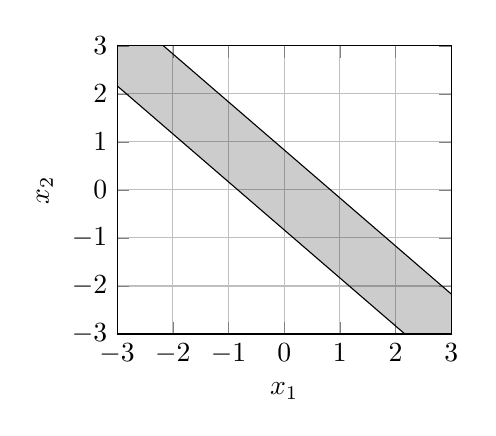
\begin{tikzpicture}
        \begin{axis}[
            scale only axis,
            width=.35\textwidth,
            % axis lines=center,
            xlabel={$x_1$},
            ylabel={$x_2$},
            ymin=-3, ymax=3,
            xmin=-3, xmax=3,
            grid,
            samples=2,
            xtick={-3,...,3},
            ytick={-3,...,3}
        ]
            \addplot[name path=A] {-x + sqrt(-ln(0.5))};
            \addplot[name path=B] {-x - sqrt(-ln(0.5))};
            \addplot[black,opacity=0.2] fill between[of=A and B];
        \end{axis}
    \end{tikzpicture}
    \hspace{.05\textwidth}
    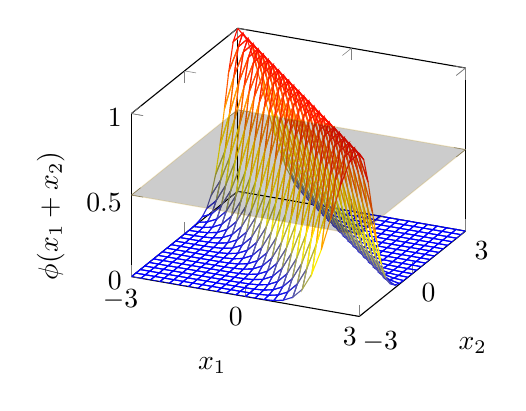
\begin{tikzpicture}
        \begin{axis}[
            scale only axis,
            width=.35\textwidth,
            ymin=-3, ymax=3,
            xmin=-3, xmax=3,
            zmin=0, zmax=1,
            xlabel={$x_1$},
            ylabel={$x_2$},
            zlabel={$\phi(x_1+x_2)$},
            samples=25,
            xtick={-3,0,3},
            ytick={-3,0,3},
            ztick={0, 1},
            extra z ticks={0.5}
        ]
            % \addplot3[
            %     name path=A,
            %     samples=2,
            %     mark=none
            % ] ({x}, {-x - sqrt(-ln(0.5))}, {0.5});
            % \addplot3[
            %     name path=B,
            %     samples=2,
            %     mark=none
            % ] ({x}, {-x + sqrt(-ln(0.5))}, {0.5});
            % \addplot3[black,opacity=0.4] fill between[of=A and B];
            \addplot3 [
                mesh,
                domain=-3:3,
                y domain=-3:3,
            ] {exp(-(x+y)^2)};
            \addplot3 [
                surf,
                fill=black,
                opacity=0.2,
                domain=-3:3,
                y domain=-3:3,
                samples=2
            ] {.5};
        \end{axis}
    \end{tikzpicture}
    \caption{Plot of hyperplanes in input space of the radial basis activation function.}
    \label{fig:week6:rbf:hyperplanes}
\end{figure}

\paragraph{Remarks:}
Notice that the radial basis function given in (\ref{eq:week6:rbf}) is differentiable and hence a suitable activation function for neural networks.
This means that if we use this activation function, we do not require hidden units in order to create a stripe configuration.

\subsection{The stripe problem without hidden units}
\label{sec:week6:stripe}
From the findings of the previous section, it follows that we could create the stripe problem with the neural network architecture from Fig. \ref{fig:week6:rbf:neuralnet} and the hyperplanes that are a result of the radial basis activation function.
Fig. \ref{fig:week6:rbf:hyperplanes} shows the hyperplanes for the initial weight configuration $w_1=w_2=1$.

We require four sample points to produce the problem, and they must be arranged in a way where the mean squared error is required to temporarily increase before it decreases.
The initial and possible goal configuration are shown in Fig. \ref{fig:week6:stripe:initialconfig}.

The depicted goal configuration can be achieved when either $w_1$ or $w_2$ changes to $-1$ whilst the other weight remains at $1$. In gradually changing the weight, some points will necessarily be misclassified. 

\begin{figure}[h]
    \centering
    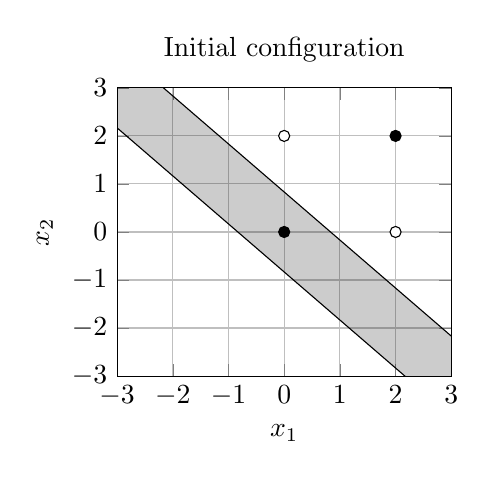
\begin{tikzpicture}
        \begin{axis}[
            scale only axis,
            width=.35\textwidth,
            title={Initial configuration},
            xlabel={$x_1$},
            ylabel={$x_2$},
            ymin=-3, ymax=3,
            xmin=-3, xmax=3,
            grid,
            samples=2,
            xtick={-3,...,3},
            ytick={-3,...,3}
        ]
            \addplot[name path=A] {-x + sqrt(-ln(0.5))};
            \addplot[name path=B] {-x - sqrt(-ln(0.5))};
            \addplot[black,opacity=0.2] fill between[of=A and B];

            \addplot[only marks, mark=o, mark options={
                fill=black,draw=black
            }] table {
                0 0
                2 2
            };
            \addplot[only marks, mark=o, mark options={
                fill=white,draw=black
            }] table {
                0 2
                2 0
            };
        \end{axis}
    \end{tikzpicture}
    \vspace{.05\textwidth}
    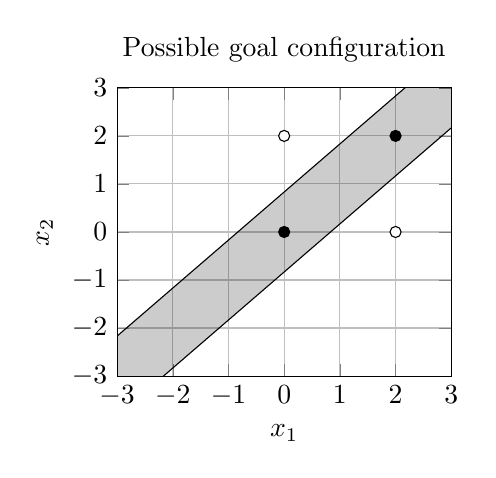
\begin{tikzpicture}
        \begin{axis}[
            scale only axis,
            width=.35\textwidth,
            title={Possible goal configuration},
            xlabel={$x_1$},
            ylabel={$x_2$},
            ymin=-3, ymax=3,
            xmin=-3, xmax=3,
            grid,
            samples=2,
            xtick={-3,...,3},
            ytick={-3,...,3}
        ]
            \addplot[name path=A] {x + sqrt(-ln(0.5))};
            \addplot[name path=B] {x - sqrt(-ln(0.5))};
            \addplot[black,opacity=0.2] fill between[of=A and B];

            \addplot[only marks, mark=o, mark options={
                fill=black,draw=black
            }] table {
                0 0
                2 2
            };
            \addplot[only marks, mark=o, mark options={
                fill=white,draw=black
            }] table {
                0 2
                2 0
            };
        \end{axis}
    \end{tikzpicture}
    \caption{Initial and possible goal configuration for the stripe problem.}
    \label{fig:week6:stripe:initialconfig}
\end{figure}

This becomes evident when graphing the error-weight surface, as shown in Fig. \ref{fig:week6:stripe:errorsurface}. 
There is no path from the initial configuration to the global minimum with a strictly decreasing error; the error must temporarily be increased (by overcoming a hill) until reaching the global minimum trough.

\begin{figure}[h]
    \centering
    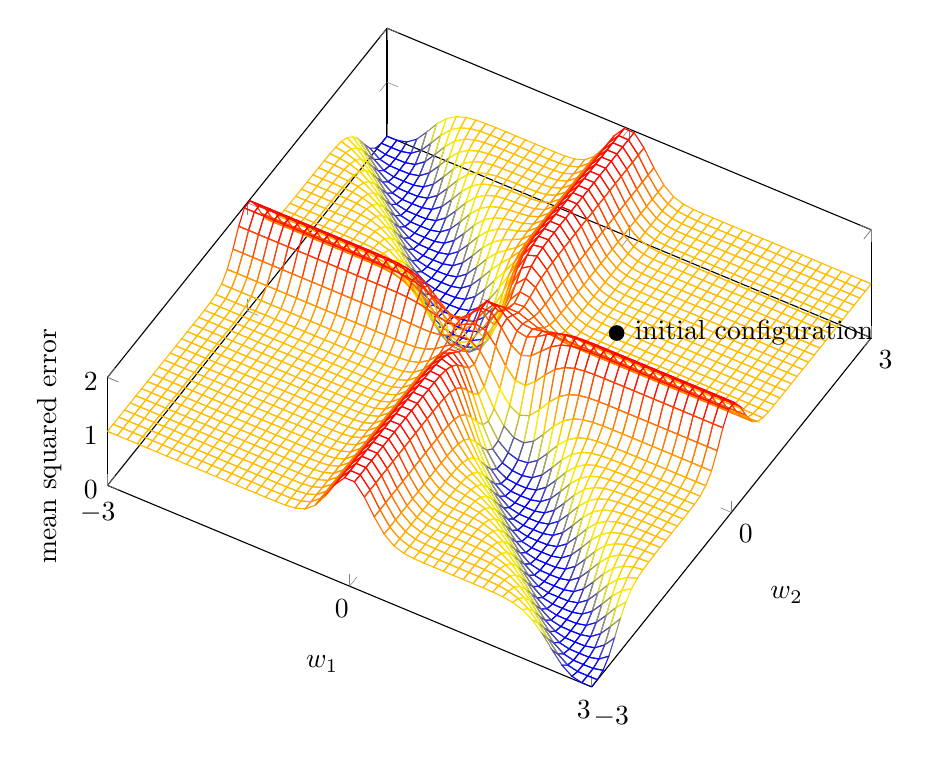
\begin{tikzpicture}
        \begin{axis}[
            scale only axis,
            width=.8\textwidth,
            ymin=-3, ymax=3,
            xmin=-3, xmax=3,
            zmin=0, zmax=2,
            xlabel={$w_1$},
            ylabel={$w_2$},
            zlabel={mean squared error},
            samples=50,
            xtick={-3,0,3},
            ytick={-3,0,3},
            ztick={0, 1, 2},
            view={30}{75}
        ]
            \addplot3 [
                mesh,
                domain=-3:3,
                y domain=-3:3
            ] {(exp(-4*x^2))^2 + (exp(-4*y^2))^2 + (1 - exp(-(2*x + 2*y)^2))^2};
            \node[label={360:{initial configuration}},circle,fill,inner sep=2pt] at (1, 1, 1) {};
        \end{axis}
    \end{tikzpicture}
    \caption{The error-weight surface of the stripe problem.}
    \label{fig:week6:stripe:errorsurface}
\end{figure}

\begin{wrapfigure}{R}{0.55\textwidth}
    \begin{tikzpicture}
        \begin{axis}[
            scale only axis,
            width = 0.4\textwidth,
            title = {Training progress},
            xlabel = {training step},
            ylabel = {loss},
            yticklabel style={/pgf/number format/.cd,fixed,precision=5}
            ]
            \addplot table {../data/week6_stripe_loss.dat};
        \end{axis}
    \end{tikzpicture}
    \caption{Loss over time during training.}
    \label{fig:week6:stripe:trainingloss}
\end{wrapfigure}

\paragraph{Training using gradient descent}
To test the above findings, this simple neural network was trained using the \texttt{keras} framework. 
As expected, the Stochastic Gradient Descent (SGD) optimizer did not achieve any noticable progress.
After 20,000 iterations, the weights were at $w_1=w_2=1.105$, i.e. they did not move to a configuration where $w_1=-w_2$ which would constitute the global minimum. 

Fig. \ref{fig:week6:stripe:trainingloss} depicts the training accuracy across the 20,000 iterations.
The only progress that was achieved was in the order of $10^{-3}$, and that was not in the direction of the global minimum.
Furthermore, the graph seems to converge to a value around $0.25$.

This means that we have found a simple example where SGD suffers the local minimum problem.

\clearpage
\subsection{Training the neural network with the shallow excitation gradient}

\begin{wraptable}{R}{0.55\textwidth}
    \begin{tabular}{c|c|c}
        point in input space & initial value & target value \\
        \hline
        $\vec{a} = \begin{bmatrix}
            0.6 \\ 0.4
        \end{bmatrix}$
        &  0.51 & 0.2 \\
        $\vec{b} = \begin{bmatrix}
            0.6 \\ 1.0
        \end{bmatrix}$
        &  0.55 & 0.8
    \end{tabular}
    \caption{Initial and target values for $\vec{a}$ and $\vec{b}$.}
    \label{table:week6:shallownet:aandb}
\end{wraptable}
Let's come back to the neural network from Sec. \ref{sec:week5:shallownet} given in Fig. \ref{fig:week5:shallownet}.
Recall the two points in input space $\vec{a}$ and $\vec{b}$ with initial and target values given in Table \ref{table:week6:shallownet:aandb}.

In order to test the behaviour of gradient descent, we will give point $\vec{b}$ a weighting four times higher than $\vec{a}$ by simply duplicating $\vec{b}$ four times in the training set which is then given by $\left\{ \vec{a}, \vec{b}, \vec{b}, \vec{b}, \vec{b}\right\}$.

The neural network's weights $w_1$ and $w_2$ were trained for 5,000 steps using \texttt{keras}. 
Note that the bias was kept constant at $b=0.45$, and the network has no activation function.
Fig. \ref{fig:week6:shallownet:trainingloss} shows the training progress over time. 
It can be seen that the gradient descent optimizer initially reduces the loss quite quickly (hence the steep slope), but around step 100, the slope becomes much more shallow.
The reason for this is that until this step, the network prioritized getting a better prediction result for $\vec{b}$, but the initial rapid improvements to the four points at $\vec{b}$ caused significant deteriorations in the predictions for point $\vec{a}$.
Fig. \ref{fig:week6:shallownet:predictions} illustrates this point, as the prediction for $\vec{a}$ first moves away from the target (it increases from 0.51, instead of decreasing to the target 0.2) before performing a sharp turn around iteration 100 after which it decreased until eventually meeting 0.2.

Finally, Fig. \ref{fig:week6:shallownet:weights} shows how the weights $w_1$ and $w_2$ were updated during the training process. It can clearly be seen that SGD does not choose the optimal way of updating weights which would be a straight line from the initial weight configuration to the final configuration.

\begin{figure}[h]
    \begin{tikzpicture}
        \begin{axis}[
            scale only axis,
            width = 0.4\textwidth,
            title = {Training progress},
            xlabel = {training step},
            ylabel = {loss},
            yticklabel style={/pgf/number format/.cd,fixed},
            scaled y ticks=false,
            ymin=0, ymax=.08
            ]
            \addplot table {../data/week6_shallow_network_loss.dat};
        \end{axis}
    \end{tikzpicture}
    \vspace{.05\textwidth}
    \begin{tikzpicture}
        \begin{axis}[
            scale only axis,
            width = 0.4\textwidth,
            title = {Initial training progress (first 1,000 steps)},
            xlabel = {training step},
            ylabel = {loss},
            yticklabel style={/pgf/number format/.cd,fixed},
            scaled y ticks=false,
            ymin=0, ymax=.08, xmax=1000
            ]
            \addplot table {../data/week6_shallow_network_loss_1000.dat};
        \end{axis}
    \end{tikzpicture}
    \caption{Loss over time during training. Notice the abrupt change in gradient which can be seen in more detail on the right.}
    \label{fig:week6:shallownet:trainingloss}
\end{figure}

\begin{figure}[h]
    \begin{tikzpicture}
        \begin{axis}[
            scale only axis,
            width = 0.4\textwidth,
            title = {Predictions for $\vec{a}$ and $\vec{b}$ over time},
            xlabel = {training step},
            ylabel = {prediction ($y$)},
            legend entries = {$y(\vec{a})$, $y(\vec{b})$},
            legend style = {at={(.97,.5)}, anchor=east}
            ]
            \addplot table {../data/week6_shallow_network_predictions_a.dat};
            \addplot table {../data/week6_shallow_network_predictions_b.dat};
        \end{axis}
    \end{tikzpicture}
    \vspace{.05\textwidth}
    \begin{tikzpicture}
        \begin{axis}[
            scale only axis,
            width = 0.4\textwidth,
            title = {Predictions in relation to each other},
            xlabel = {$y(\vec{a})$},
            ylabel = {$y(\vec{b})$}
            ]
            \addplot table {../data/week6_shallow_network_predictions.dat};
        \end{axis}
    \end{tikzpicture}
    \caption{Changes in the predictions of $\vec{a}$ and $\vec{b}$ during the training process.}
    \label{fig:week6:shallownet:predictions}
\end{figure}

\begin{figure}[h]
    \begin{tikzpicture}
        \begin{axis}[
            scale only axis,
            width = 0.4\textwidth,
            title = {Changes in weights during training \\ (first 1,000 steps)},
            title style={align=center},
            xlabel = {training step},
            ylabel = {weight value},
            legend entries = {$w_1$, $w_2$},
            legend style = {at={(.97,.5)}, anchor=east}
            ]
            \addplot table {../data/week6_shallow_network_weight_0.dat};
            \addplot table {../data/week6_shallow_network_weight_1.dat};
        \end{axis}
    \end{tikzpicture}
    \vspace{.05\textwidth}
    \begin{tikzpicture}
        \begin{axis}[
            scale only axis,
            width = 0.4\textwidth,
            title = {Weights in relation to each other},
            xlabel = {$w_1$},
            ylabel = {$w_2$}
            ]
            \addplot table {../data/week6_shallow_network_weights.dat};
        \end{axis}
    \end{tikzpicture}
    \caption{Changes in weights during the training process.}
    \label{fig:week6:shallownet:weights}
\end{figure}

\section{Week 11}
\subsection{Defining unrealizable regions}
An \textit{unrealizable region} is a subspace of the output space that cannot be attained. 
Consider a neural network architecture expressed as the function $\vec{f}(\vec{x}; \vec{W}_1, \dots, \vec{W}_n)$ that takes the weight configurations $\vec{W}$ for each layer as a parameter.
Given the sample $\langle \vec{x}, \vec{y}\rangle$ where $\vec{x}$ lies in input space and $\vec{y}$ in output space, we say that $\vec{y}$ is \textit{strongly unrealizable} iff there exists no weight configuration $\vec{W}_1,\dots,\vec{W}_n$ such that $\vec{f}(\vec{x};\vec{W}_1,\dots,\vec{W}_n)=\vec{y}$. 

A point is \textit{weakly unrealizable} for particular training algorithm if that algorithm cannot achieve a weight configuration such that $\vec{f}(\vec{x};\vec{W}_1,\dots,\vec{W}_n)=\vec{y}$.

\subsection{The problem of non-orthogonal weight gradients}
\label{sec:week11:orthogonal}

\begin{wrapfigure}{r}{.5\textwidth}
    \centering
    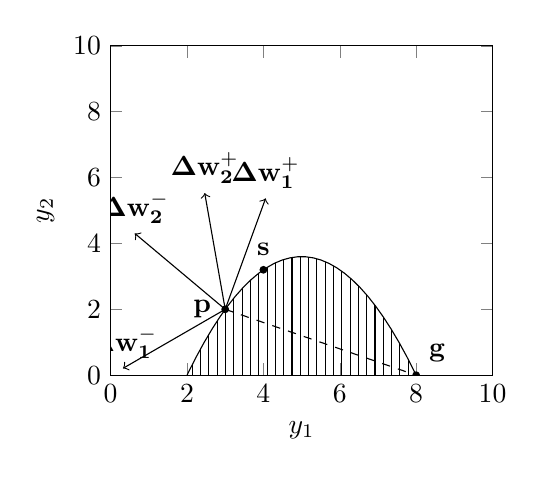
\begin{tikzpicture}
        \begin{axis}[
            scale only axis,
            width=.4\textwidth,
            xmin=0, xmax=10,
            ymin=0, ymax=10,
            xlabel = {$y_1$},
            ylabel = {$y_2$}
        ]
            \path[name path=axis] (axis cs:0,0) -- (axis cs:1,0);
            \addplot[name path=unrealizable, domain=0:10, samples=50] {(-2*x^2 + 20*x - 32)/5};
            \addplot[
                pattern=vertical lines,
                pattern color=black
            ] fill between[of=unrealizable and axis];

            \coordinate (p) at (3, 2);
            \draw[->] (p) -- ++(70:1.5cm) node[above] {$\vec{\Delta w_1^+}$};
            \draw[->] (p) -- ++(100:1.5cm) node[above] {$\vec{\Delta w_2^+}$};
            \draw[->] (p) -- ++(140:1.5cm) node[above] {$\vec{\Delta w_2^-}$};
            \draw[->] (p) -- ++(210:1.5cm) node[above] {$\vec{\Delta w_1^-}$};
            \node[label={180:{$\vec{p}$}}, circle, fill, inner sep=1pt] at (p) {};

            \coordinate (s) at (4, 16/5);
            \coordinate (g) at (8, 0);
            \draw[dashed] (p) -- (g);
            \node[label={90:{$\vec{s}$}}, circle, fill, inner sep=1pt] at (s) {};
            \node[label={45:{$\vec{g}$}}, circle, fill, inner sep=1pt] at (g) {};
        \end{axis}
    \end{tikzpicture}
    \caption{Weight changes in output space.}
    \label{fig:week11:orthogonal}
\end{wrapfigure}

Consider a neural network with two weights $w_1$ and $w_2$, as well as two outputs $y_1$ and $y_2$. 
Figure \ref{fig:week11:orthogonal} depicts a particular configuration in output space, showing an unrealizable region as well as how changes in the weights will affect the output\footnote{The diagram displays a made-up scenario that does not correspond to an actual experiment.}. 
Note that in this example, $\vec{\Delta w^+} \neq -\vec{\Delta w^-}$, i.e. changing a weight in the negative direction does \textit{not} result in a change in the opposite direction because the problem is inherently non-linear. 

Furthermore, the vector $\vec{\Delta w^+}$ is \textit{not} the same as the partial derivative $\frac{\delta w}{\delta \vec{y}}$. 
Instead, the value of $\vec{\Delta w^+}$ was obtained by calculating the neural network's output, substituting $w$ for $w+\alpha$ for some small $\alpha$. 
Similarly, $\vec{\Delta w^-}$ was obtained by calculating the output where $w$ is $w-\alpha$. 

The current configuration produces point $\vec{p}$ in output space. 
Say we want to achieve the sub-goal $\vec{s}$ in the next step.
What change in $w_1$ and $w_2$ will get us closest to $\vec{s}$?

\paragraph{Treating the problem as being linear}
How do we define \textit{linear}, and how would we solve this?

\paragraph{Brute-force all assignments}
We could calculate the output of the network for all possible assignments of the weights. 
Every weight $w$ will be tested with the values $w-\alpha$, $w$, and $w+\alpha$. 
The limitation of this technique is that the time complexity will be $\mathcal{O}(3^n)$ where $n$ is the number of weights, and this calculation has to be carried out at each step. 

\paragraph{Random assignments}
Instead, we could test a subset of the $3^n$ possible assignments. For example, we could randomly generate assignments (each weight $w$ being either $w-\alpha$, $w$, or $w+\alpha$) until we find one that is \textit{good enough} according to some previously defined stopping condition. 


\subsection{Controlling properties of the RBF stripe problem}
\subsubsection{Width of the basin}
In order to control the width of the basin, we need to control the thickness of the RBF activation function. 
We introduce the parameter $\epsilon$ which will affect the width of the RBF function from (\ref{eq:week6:rbf}), now given as
\begin{equation}
    \label{eq:week11:rbf_thickness}
    \phi(x; \epsilon) = e^{-\epsilon x^2}.
\end{equation}
Figure \ref{fig:week11:rbf_thickness:plot} depicts a plot of the RBF for $\epsilon=10$, showing clearly that the resulting function has a thinner graph as compared to Figure \ref{fig:week6:rbf:plot} where $\epsilon=1$.
Furthermore, Figure \ref{fig:week11:stripe:errorsurface:thin} shows that the error-weight surface for the stripe problem given in Section \ref{sec:week6:stripe} has a narrower minimum basin using the thinner RBF as compared to Figure \ref{fig:week6:stripe:errorsurface}.
\begin{figure}[h]
    \centering
    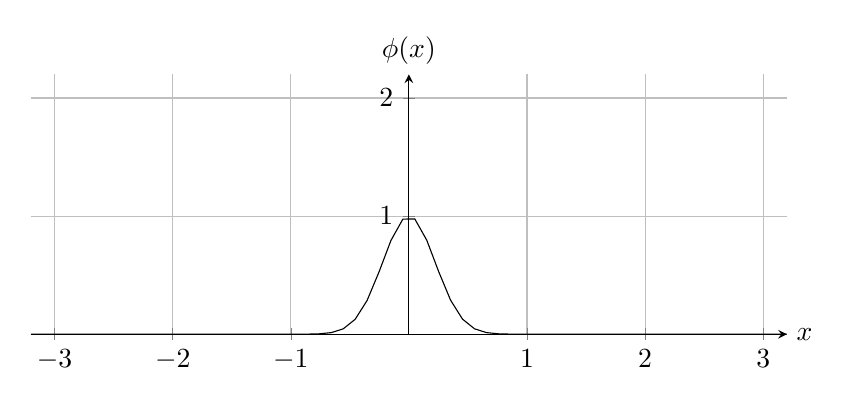
\begin{tikzpicture}
        \begin{axis}[
            x=1.5cm,
            y=1.5cm,
            axis lines=center,
            xlabel={$x$}, xlabel style={anchor=west},
            ylabel={$\phi(x)$}, ylabel style={anchor=south},
            ymin=0, ymax=2.2,
            xmin=-3.2, xmax=3.2,
            grid,
            samples=100,
            xtick={-3,...,3},
            ytick={0, 1, 2}
        ]
            \addplot[black] {exp(-x*x*10)};
        \end{axis}
    \end{tikzpicture}
    \caption{Plot of the radial basis activation function with $\epsilon=10$.}
    \label{fig:week11:rbf_thickness:plot}
\end{figure}
\begin{figure}[h]
    \centering
    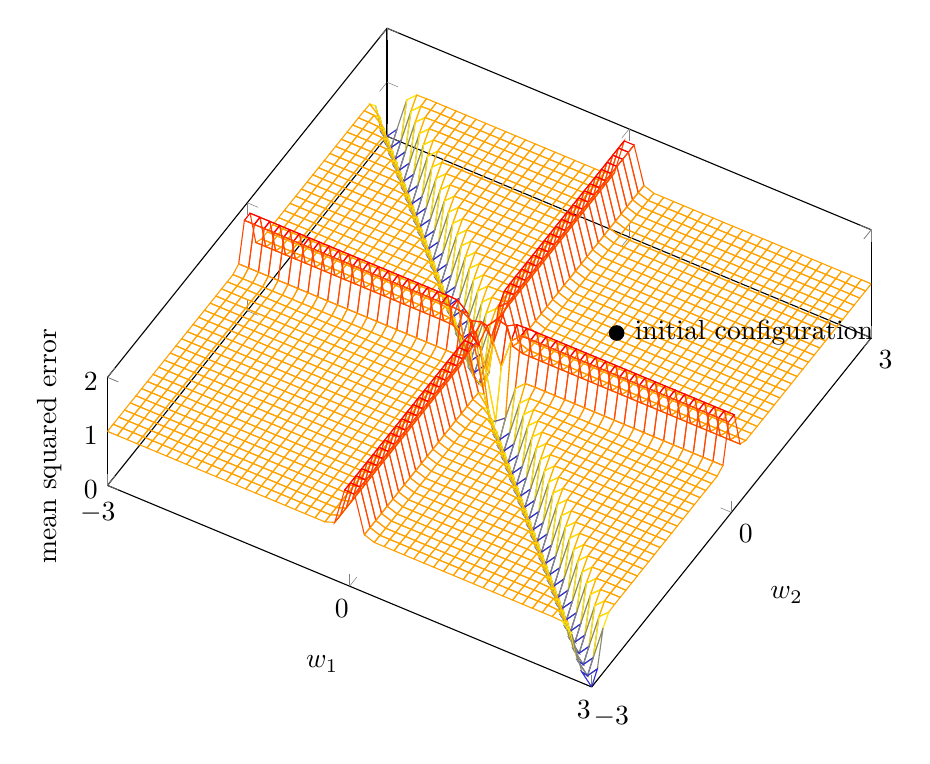
\begin{tikzpicture}
        \begin{axis}[
            scale only axis,
            width=.8\textwidth,
            ymin=-3, ymax=3,
            xmin=-3, xmax=3,
            zmin=0, zmax=2,
            xlabel={$w_1$},
            ylabel={$w_2$},
            zlabel={mean squared error},
            samples=50,
            xtick={-3,0,3},
            ytick={-3,0,3},
            ztick={0, 1, 2},
            view={30}{75}
        ]
            \addplot3 [
                mesh,
                domain=-3:3,
                y domain=-3:3
            ] {(exp(-4*x^2*10))^2 + (exp(-4*y^2*10))^2 + (1 - exp(-(2*x + 2*y)^2*10))^2};
            \node[label={360:{initial configuration}},circle,fill,inner sep=2pt] at (1, 1, 1) {};
        \end{axis}
    \end{tikzpicture}
    \caption{The error-weight surface of the stripe problem with a narrower basin.}
    \label{fig:week11:stripe:errorsurface:thin}
\end{figure}

\subsubsection{Guaranteeing a finite number of solutions with MSE of zero}

For the stripe problem as defined in Section \ref{sec:week6:stripe}, there exists no real-valued weight configuration that leads to a mean squared error of 0. 
This is because the activation function is always greater than 0. In fact, the range of $\phi$ is the interval $\left(0, 1\right]$.

We will set the training dataset as shown in Table \ref{table:week11:dataset}. 
Essentially, the data is the same as shown in Figure \ref{fig:week6:stripe:initialconfig}, except that the targets of $0$ have been adapted to slightly higher values.

\begin{table}[h!]
    \centering
    \begin{tabular}{c|c|c}
        input ($\vec{x}$) & target output ($\vec{y}$) & initial output \\
        \hline
        $\begin{bmatrix} 0 \\ 0 \end{bmatrix}$
        & 1 & 1
        \\
        $\begin{bmatrix} 2 \\ 2 \end{bmatrix}$
        & 1 & $\phi\left( 4 \right)$
        \\
        $\begin{bmatrix} 0 \\ 2 \end{bmatrix}$
        & $\phi\left( 2 \right)$ & $\phi\left( 2 \right)$
        \\
        $\begin{bmatrix} 2 \\ 0 \end{bmatrix}$
        & $\phi\left(2 \right)$ & $\phi\left( 2 \right)$
    \end{tabular}
    \caption{Initial and target values for $\vec{a}$ and $\vec{b}$.}
    \label{table:week11:dataset}
\end{table}

In the initial configuration, $w_1=w_2=1$, so the mean squared error is
\begin{align*}
    MSE &= \sum_i{\left(f(\vec{x}_i) - \vec{y}_i\right)^2}
    \\ &= \left(1 - 1 \right)^2 + \left(e^{-8\epsilon} - 1 \right)^2 + \left(\phi\left( \sqrt{2} \right) - \phi\left( \sqrt{2} \right) \right)^2 + \left(\phi\left( \sqrt{2} \right) - \phi\left( \sqrt{2} \right) \right)^2.
    \\ &= \left(e^{-8\epsilon} - 1 \right)^2.
\end{align*}

If we consider the weight configuration $w_1=1$ and $w_2=-1$, we obtain
\begin{align*}
    MSE &= \left(f\left( \begin{bmatrix} 0 \\ 0 \end{bmatrix} \right) - 1 \right)^2 + \left(f\left( \begin{bmatrix} 2 \\ 2 \end{bmatrix} \right) - 1 \right)^2 + \left(f\left( \begin{bmatrix} 0 \\ 2 \end{bmatrix} \right) - \phi\left( \sqrt{2} \right) \right)^2 + \left(f\left( \begin{bmatrix} 2 \\ 0 \end{bmatrix} \right) - \phi\left( \sqrt{2} \right) \right)^2
    \\ &= \left(\phi \left( 0 + 0 \right) - 1 \right)^2 + \left(\phi \left( 2 - 2 \right) - 1 \right)^2 + \left(\phi \left( 0 - 2 \right) - \phi\left( 2 \right) \right)^2 + \left(\phi \left( 2 - 0 \right) - \phi\left( 2 \right) \right)^2
    \\ &= \left(\phi \left( 0 \right) - 1 \right)^2 + \left(\phi \left( 0 \right) - 1 \right)^2 + \left(\phi \left( - 2 \right) - \phi\left( 2 \right) \right)^2 + \left(\phi \left( 2 \right) - \phi\left( 2 \right) \right)^2.
\end{align*}
Noticing that $\phi(0)=1$ and $\phi(x)=\phi(-x)$ for any $x$, we obtain $MSE=0$. 
In fact, there are only two unique weight configurations that lead to $MSE=0$; these are $\vec{w}=\begin{bmatrix}1\\-1 \end{bmatrix}$ and $\vec{w}=\begin{bmatrix}-1\\ 1 \end{bmatrix}$, so these are the only global minima in the error-weight surface. 
Incidentally, the solutions do \textit{not} depend on the parameter $\epsilon$ for the activation function $\phi(x)$ provided $\epsilon \neq 0$. 

\paragraph{Remarks:}
To improve, it might be better to instead use a so-called \textit{non-analytic smooth function} that is similar to the RBF activation function, except that its range includes zero. 
One example of such a function is the \textit{bump function}\footnote{\url{https://en.wikipedia.org/wiki/Bump_function}}. 
This will be investigated in the next semester.

\section{Week 12}

\subsection{Assumptions on linearity}
Using the notation from Section \ref{sec:week11:orthogonal}, we make the following assumptions: 
\begin{itemize}
    \item For a given weight $w$, the change that $w+\alpha$ for a small $\alpha$ will elicit in output space, denoted $\vec{\Delta w^+}$, is \textit{linearly independent} of $\vec{\Delta w^-}$ in the local context of $\alpha$. 
    
    It follows that $\vec{\Delta w^+}$ and $\vec{\Delta w^-}$ are usually not collinear. 
    \item Given two weights $w_1$ and $w_2$, we assume that the pairs $\langle \vec{\Delta w_1^+, \Delta w_2^+} \rangle$, $\langle \vec{\Delta w_1^+, \Delta w_2^-} \rangle$, $\langle \vec{\Delta w_1^-, \Delta w_2^+} \rangle$, and $\langle \vec{\Delta w_1^-, \Delta w_2^-} \rangle$ obey the rules of vector sums in the context of $\alpha$.

    \item For our purposes, a linear combination $\vec{\mathcal{L}}$ of two vectors $\vec{\Delta w_1}$ and $\vec{\Delta w_2}$ is defined as
        $$\vec{\mathcal{L}}(\vec{\Delta w_1}, \vec{\Delta w_2}) = c_1 \vec{\Delta w_1} + c_2 \vec{\Delta w_2}$$
        where $c_1$ and $c_2$ are real-valued scalars such that \textcolor{red}{$0 \leq c_i \leq 1$ for both $i$}.
    \item The weight update corresponding to a linear combination $\vec{\mathcal{L}}(\vec{\Delta w_1^+}, \vec{\Delta w_2^+})$ is $w_1 \leftarrow w_1 + c_1 \alpha$ and $w_2 \leftarrow w_2 + c_2 \alpha$. 
        
    When considering weight changes in the negative direction, i.e. $\vec{\Delta w_1^-}$, the corresponding weight update will be $w_1 \leftarrow w_1 - c_1 \alpha$.
    
    Note that the update $w \leftarrow w + c \alpha$ is based on the assumption that the mapping between weight and output space is \textit{linear} in the context of $\alpha$. 
    This might not be the case and yield inaccurate results, so instead we might need to modify the algorithm to carry out a linear search instead to find what change in $w$ will yield a vector of length $c \norm{\vec{\Delta w}}$.
    \item It does not make sense to compute a linear combination of $\vec{\Delta w^+}$ and $\vec{\Delta w^-}$ for the same weight $w$ because this does not correspond to a meaningful weight update. 
\end{itemize}

\paragraph{Defining output space}
The output space is only defined for networks with one output neuron. Each dimension corresponds to the activation of the output neuron for a training sample, so the number of dimensions of the output space is the number of training samples.

\paragraph{Question}
I understand how we aim to achieve a subgoal point using orthogonalization (Gram-Schmidt) and vector sums, \textit{but how do we select the subgoal point?}

Do we just choose the subgoal to be, for example, one tenth of the way to the goal, i.e. the subgoal is lying on the goal line?
Then if we deviate from the goal line this is because our local assumptions of linearity aren't 100 percent accurate (but that might not be too bad, as long as we don't deviate too much).
The deviation from the goal line would then be described as a weakly unrealizable region.

If it is impossible to achieve a point on the goal line (because all gradients point away from it, like in Figure \ref{fig:week11:orthogonal}), we could just go for the weight change that makes the maximum fractional progress, and only change that one weight. 
Otherwise we could devise some sort of informed search that will yield the weight combination with the maximum fractional progress\footnote{It is important to notice that while the change in weight $\alpha$ is the same for each weight, the vector $\vec{\Delta w}$ in output space might not have the same magnitude as the others. This means that potentially a combination of weights might lead to a better fractional progress than just changing only one weight.}. 




\section{Christmas vacation}

\subsection{Modifying the loss function to include the deviation from the goal line}
It would be interesting to investigate how a neural network would train with a loss function defined as
$Loss = MSE + d^2$ where $d$ is the deviation from the goal line. More formally, given 
\begin{itemize}
    \item the target output $\vec{y}$,
    \item the initial actual output $\vec{\hat{y}}_0$ when the training was started, and
    \item the actual output at the current step $i$, denoted $\vec{\hat{y}}_i$,
\end{itemize}
we define $d$ as the shortest distance from the point $\vec{\hat{y}}_i$ in output space to the line going through the points $\vec{\hat{y}}_0$ and $\vec{y}$ (the \textit{goal line} in output space).

\section{Semester 2, week 3}

\subsection{The `cheating' technique}
\paragraph{Motivation}
The neural surfer must be able to perform two main tasks: 
\begin{enumerate*}[label=(\roman*)]
    \item setting the subgoals and
    \item achieving the subgoals.
\end{enumerate*}
The `cheating' technique pertains to the latter task; it can be used in order to determine whether and to what extent the training regimes are \textit{capable} of realising each subgoal.
The idea is that splitting the problem into two parts will facilitate an easier debugging process of the approaches in terms of isolating pain points and performance issues.

The technique allows us to analyze the following questions:
\begin{itemize}
    \item How well is the approach getting to the subgoals?
    \item How good is the state the approach ends up in when it achieves the subgoal?
\end{itemize}

\paragraph{Achieving a subgoal}
One important question that must be answered is what constitutes realising a subgoal. 
For the purpose of this experiment, we will assume that achieving half of the distance to the subgoal constitutes as `achieving' it. 
However, it is important to note that for further investigation, it might be worthwhile to look at other values, or even functions that give a specific threshold for each subgoal.

\paragraph{Procedure}
The steps below explain the methodology of this technique, for $n$ subgoals.
\begin{enumerate}
    \item Determine the point in weight space $\vec{w_{n+1}}$ that corresponds to the target in output space (i.e. the global minimum on the error-weight surface). 
        
        This can be done either by
        \begin{enumerate*}[label=(\roman*)]
            \item analytically finding the global minimum of the error-weight space if the network architecture is simple enough; or
            \item running gradient descent from many random initial configurations in order to find the global minimum.
        \end{enumerate*}
    
    \item Draw a straight line from the initial weight configuration $\vec{w_0}$ to the target configuration in weight space $\vec{w_{n+1}}$.
        This is the \textit{goal line}.
    
    \item Put $n$ points on the goal line, $\vec{w_1}, \vec{w_2}, \dots, \vec{w_n}$, equidistant between $\vec{w_0}$ and $\vec{w_{n+1}}$. 
        Determine the corresponding points $\vec{\hat{y}_1}, \vec{\hat{y}_2}, \dots, \vec{\hat{y}_n}$ in output space.
    \item Let $i=0$. Starting at weight configuration $\vec{w_i}$, perform the particular neural network training technique until achieving a point $\vec{p}$ in output space where $\norm{\vec{p} - \vec{\hat{y}_{i+1}}} \leq \frac{1}{2} \norm{\vec{\hat{y}_i} - \vec{\hat{y}_{i+1}}}$, i.e. at least half of the distance to the next subgoal is achieved.
    \item Repeat the previous step for $i=1, 2, \dots, n$.
    \item Perform the particular neural network training technique to achieve a configuration sufficiently close to the goal, $\vec{y}$. 
\end{enumerate}

\begin{figure}[h!]
    \centering
    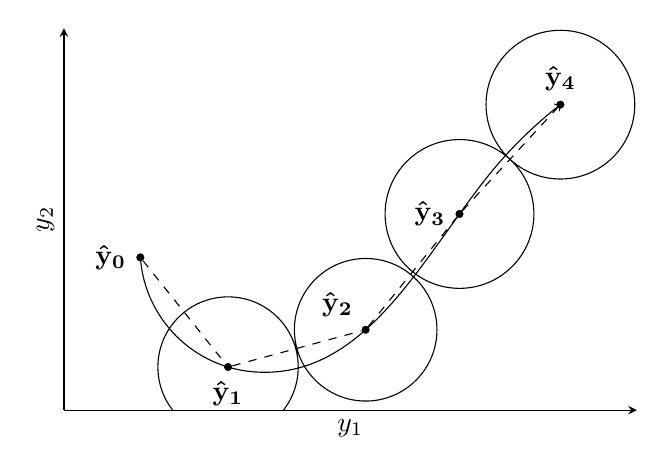
\begin{tikzpicture}
        \begin{axis}[
            scale only axis,
            width=.6\textwidth,
            height=.4\textwidth,
            xmin=0, xmax=15,
            ymin=0, ymax=10,
            xlabel={$y_1$},
            ylabel={$y_2$},
            ticks=none,
            axis x line=bottom,
            axis y line=left
        ]
            \coordinate (initial) at (2, 4);
            \coordinate (goal) at (13, 8);

            \draw[->,
                postaction={
                    decorate,
                    decoration={
                        markings,% switch on markings 
                        mark=% actually add a mark
                            between positions 0 and 1 step 0.9999/4
                            with
                            {
                                \node[circle,fill,inner sep=1pt](w-\pgfkeysvalueof{/pgf/decoration/mark info/sequence number}){};
                            }
                    }
                }
            ] (initial) (initial) to[curve through={(5,1) .. (11,6)}] (goal);

            \node[label={180:{$\vec{\hat{y}_0}$}}, circle, fill, inner sep=1pt] at (w-1) {};
            \node[label={270:{$\vec{\hat{y}_1}$}}, circle, fill, inner sep=1pt] at (w-2) {};
            \node[label={135:{$\vec{\hat{y}_2}$}}, circle, fill, inner sep=1pt] at (w-3) {};
            \node[label={180:{$\vec{\hat{y}_3}$}}, circle, fill, inner sep=1pt] at (w-4) {};
            \node[label={90:{$\vec{\hat{y}_4}$}}, circle, fill, inner sep=1pt] at (w-5) {};

            \draw
                let
                    \p1 = ($(w-2) - (w-1)$),
                    \p2 = ($(w-3) - (w-2)$),
                    \p3 = ($(w-4) - (w-3)$),
                    \p4 = ($(w-5) - (w-4)$),
                    \n1 = {veclen(\x1, \y1)/2},
                    \n2 = {veclen(\x2, \y2)/2},
                    \n3 = {veclen(\x3, \y3)/2},
                    \n4 = {veclen(\x4, \y4)/2}
                in
                    (w-2) circle (\n1)
                    (w-3) circle (\n2)
                    (w-4) circle (\n3)
                    (w-5) circle (\n4);
            
            \draw[dashed]
                (w-1) -- (w-2)
                (w-2) -- (w-3)
                (w-3) -- (w-4)
                (w-4) -- (w-5);
            

        \end{axis}
    \end{tikzpicture}
    \caption{The `cheating' technique for $n=3$. The circles around each point indicate the threshold that constitutes `achieving' a particular point. The radius of the circle around point $\vec{\hat{y}_i}$ is $\frac{1}{2} \norm{\vec{\hat{y}_i}-\vec{\hat{y}_{i-1}}}$ for $i=1, \dots, n+1$; hence the circles are not necessarily identical in size.} 
    \label{fig:s2week3:cheat}
\end{figure}

\bibliographystyle{apalike}
\bibliography{bibliography}

\end{document}